% ----- Conclusion -----

\section{Conclusion}

As seen in the previous sections, we have been able to implement different
algorithm to solve the Maximum Edge Weight Clique problem. We will be able to
compare the different algorithms and to determine which one is the most
efficient depending on the number of vertices and the connectivity of the graph.
\bigskip

Since the MEWC problem is NP-hard, it is not possible to find a solution in
polynomial time. We have therefore tried to optimize the solution of the problem
by trying to find the most efficient algorithm to solve the problem in the best
way.
\bigskip

Among the different criteria that we will study when comparing these algorithms. We have the \textbf{speed of the results} obtained. This last one is important because the application of the MEWC on different real cases can be subject to certain time constraints. It is obvious that finding the best possible solution would be preferable but as we have seen with the exact, on a large number of vertices, we would need several generations which is not tenable to solve it. This is why we have studied other algorithms that present some alternatives. We are now going to compare them in more detail on the speed of the results obtained. \bigskip

To evaluate this, we will focus on two points: their theoretical complexity but also their execution time in practice that we have done. Note that this comparison is made on randomly generated graphs and therefore presents a general case, but each application case must be seen from a different angle and it is necessary to redo a study. \bigskip

\begin{itemize}
    \item \textbf{Complexity} : As we compare the theorical complexity of the algorithms in general, we obtain : \bigskip
    
    Exact (O($n^2\sqrt[3]{3}^n$)) $>$ Grasp (O($n^6$)) $>$ Local Search (O($n^5$)) $>$ Constructive (O($n^2$)) \bigskip

    We can observe it on the figure \ref{fig:theorical_algorithm_complexity}:

    \begin{figure}[H]
        \centering
        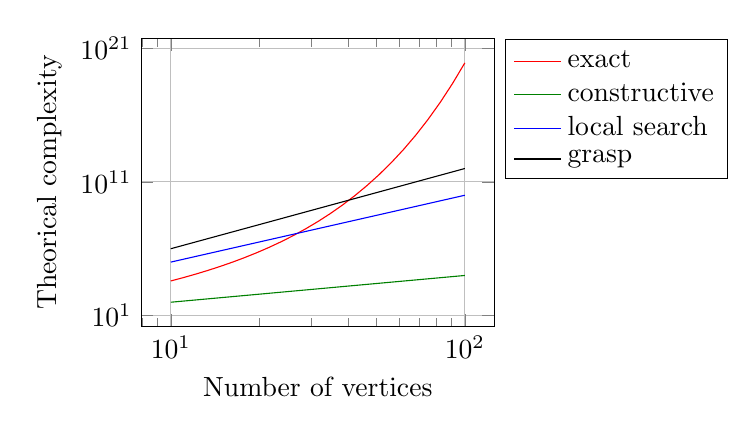
\begin{tikzpicture}
            \begin{loglogaxis}[
                    xlabel = Number of vertices,
                    ylabel = Theorical complexity,
                    legend pos = outer north east,
                    grid = major,
                    width = 0.5\textwidth,
                    legend cell align = {left},
                ]
                \addplot[Red, domain=10:100] {x^2*3^(x/3)};
    
                \addplot[Green, domain=10:100] {x^2};
    
                \addplot[Blue, domain=10:100] {x^5};
    
                \addplot[Black, domain=10:100] {x^6};
    
    
                \addlegendentry{test}
    
                \legend{exact, constructive, local search, grasp}
            \end{loglogaxis}
        \end{tikzpicture}
        \caption{Theorical omplexity of the algorithm in function of the number of vertices.}
        \label{fig:theorical_algorithm_complexity}
    \end{figure}
    
    Since the complexity will vary depending on the connectivity and degeneracy of the graph we will look at the execution time for each graph.
    
    \item \textbf{Execution time} : \bigskip
    
    You can find the execution time in the different experimental parts that we have done before in our report. We get the same results. \bigskip
    
    Exact on figure \ref{fig:exact_time} $>$ Grasp on figure \ref{fig:grasp_time} $>$ Local Search on figure \ref{fig:local_search_time} $>$ Constructive on figure \ref{fig:constructive_time}.
\end{itemize}

Another important criterion to consider is the precision of the results you are looking for, in a real application case, for example let's take our example from figure \ref{fig:applications_example}. You don't necessarily need to get the best possible click, but a slightly worse one will do just fine. The different algorithms we have studied have different levels of expectation in terms of usability results. \bigskip

To evaluate this, we will compare the percentage of the solution based on the exact one(because it always gives the best result) with different level of connectivity. \bigskip

\begin{figure}[H]
    \centering
    \begin{tikzpicture}
        \begin{axis}[
                xlabel = Number of vertices,
                ylabel = \% of solution based on exact,
                legend pos = outer north east,
                grid = major,
                width = 0.5\textwidth,
                legend cell align = {left},
            ]
            \addplot[Red, error bars/.cd, y dir=both, y explicit]
            table[x index=0, y index=1] {experiment_data/accuracy_avg_exact.dat};

            \addplot[Green, error bars/.cd, y dir=both, y explicit]
            table[x index=0, y index=1] {experiment_data/accuracy_avg_constructive_25.dat};

            \addplot[Blue, error bars/.cd, y dir=both, y explicit]
            table[x index=0, y index=1] {experiment_data/accuracy_avg_local_search_25.dat};

            \addplot[Black, error bars/.cd, y dir=both, y explicit]
            table[x index=0, y index=1] {experiment_data/accuracy_avg_grasp_25.dat};

            \addlegendentry{test}

            \legend{exact, constructive, local search, grasp}
        \end{axis}
    \end{tikzpicture}
    \caption{\% of solution based on the exact of the different algorithm for 25\% of connectivity.}
    \label{fig:algorithm_25_accuracy}
\end{figure}


For this experiment, we generated 10 random graphs with 10 to 100 vertices to find an average \% for 25\% of connectivity. The connectivity is the percentage of chance that 2 vertices are linked. The results are shown in figure \ref{fig:algorithm_25_accuracy}. At each number of vertices, an average clique weight is calculated, and converted to \% based on the result obtained with the exact algorithm. \bigskip

We can see that the exact algorithm has the best \% of solution. Grasp is second in terms of solution quality and is efficient with few vertices. Local search is third, and constructive is last. The solution quality tends to decrease as the number of vertices increases. \bigskip

Here is the average of the correct solution for each algorithms with 25\% of connectivity: \bigskip

\begin{center}
    \rowcolors{2}{gray!10}{gray!30}
    \begin{tabular}{|c|c|}
        \hline
        \textbf{Algorithms} & \textbf{Average \% of solution based on exact}                         \\
        \hline
        Exact & 100\% \\
        Grasp & 92.38\% \\
        Local Search & 76.65\% \\
        Constructive & 56.87\% \\
        \hline
    \end{tabular}
    \rowcolors{1}{}{}
\end{center}

We do exactly the same with 50\% connectivity:

\begin{figure}[H]
    \centering
    \begin{tikzpicture}
        \begin{axis}[
            xlabel = Number of vertices,
            ylabel = \% of solution based on exact,
                legend pos = outer north east,
                grid = major,
                width = 0.5\textwidth,
                legend cell align = {left},
            ]
            \addplot[Red, error bars/.cd, y dir=both, y explicit]
            table[x index=0, y index=1] {experiment_data/accuracy_avg_exact.dat};

            \addplot[Green, error bars/.cd, y dir=both, y explicit]
            table[x index=0, y index=1] {experiment_data/accuracy_avg_constructive_50.dat};

            \addplot[Blue, error bars/.cd, y dir=both, y explicit]
            table[x index=0, y index=1] {experiment_data/accuracy_avg_local_search_50.dat};

            \addplot[Black, error bars/.cd, y dir=both, y explicit]
            table[x index=0, y index=1] {experiment_data/accuracy_avg_grasp_50.dat};

            \addlegendentry{test}

            \legend{exact, constructive, local search, grasp}
        \end{axis}
    \end{tikzpicture}
    \caption{\% of solution based on the exact of the different algorithm for 50\% of connectivity.}
    \label{fig:algorithm_50_accuracy}
\end{figure}

We can observe the same results as in figure \ref{fig:algorithm_25_accuracy} for 25\%. The trends of the curves and the rankings of the algorithms are the same as before. However, we notice that the performances are better and we can see it easily with the graph of averages. \bigskip

Here is the average of the correct solution for each algorithms with 50\% of connectivity: \bigskip

\begin{center}
    \rowcolors{2}{gray!10}{gray!30}
    \begin{tabular}{|c|c|}
        \hline
        \textbf{Algorithms} & \textbf{Average \% of solution based on exact}                         \\
        \hline
        Exact & 100\% \\
        Grasp & 91.6\% \\
        Local Search & 77.45\% \\
        Constructive & 63.34\% \\
        \hline
    \end{tabular}
    \rowcolors{1}{}{}
\end{center}

We do exactly the same with 75\% connectivity:

\begin{figure}[H]
    \centering
    \begin{tikzpicture}
        \begin{axis}[
            xlabel = Number of vertices,
            ylabel = \% of solution based on the exact,
                legend pos = outer north east,
                grid = major,
                width = 0.5\textwidth,
                legend cell align = {left},
            ]
            \addplot[Red, error bars/.cd, y dir=both, y explicit]
            table[x index=0, y index=1] {experiment_data/accuracy_avg_exact.dat};

            \addplot[Green, error bars/.cd, y dir=both, y explicit]
            table[x index=0, y index=1] {experiment_data/accuracy_avg_constructive_75.dat};

            \addplot[Blue, error bars/.cd, y dir=both, y explicit]
            table[x index=0, y index=1] {experiment_data/accuracy_avg_local_search_75.dat};

            \addplot[Black, error bars/.cd, y dir=both, y explicit]
            table[x index=0, y index=1] {experiment_data/accuracy_avg_grasp_75.dat};

            \addlegendentry{test}

            \legend{exact, constructive, local search, grasp}
        \end{axis}
    \end{tikzpicture}
    \caption{\% of solution based on the exact of the different algorithm for 75\% of connectivity.}
    \label{fig:algorithm_75_time}
\end{figure}

The results obtained are identical to those for lower connectivities. We can note the confirmation that the accuracy of the results improves when the connectivity is stronger, which is a point that should be taken into account in some application cases. The connectivity will not have any importance on the accuracy ranking of each algorithm. \bigskip

Here is the average of the correct solution for each algorithms with 75\% of connectivity: \bigskip

\begin{center}
    \rowcolors{2}{gray!10}{gray!30}
    \begin{tabular}{|c|c|}
        \hline
        \textbf{Algorithms} & \textbf{Average \% of solution based on exact}                         \\
        \hline
        Exact & 100\% \\
        Grasp & 94.67\% \\
        Local Search & 85.51\% \\
        Constructive & 73.69\% \\
        \hline
    \end{tabular}
    \rowcolors{1}{}{}
\end{center}

In the end, we can conlude that each algorithm has its own advantages and disadvantages. \bigskip

The exact algorithm is able to find the optimal solution for the MEWC, but it can take a significant amount of time to do so, particularly as the number of vertices and connectivity in the problem increases. \bigskip

On the other hand, a constructive algorithm is much faster in finding a solution, but it may not necessarily result in the most optimal solution. This algorithm is a good choice when the number of vertices is large and a quick solution is needed. \bigskip

A local search algorithm is a good compromise between accuracy and time. It will give a better result than the constructive one and will stay in an acceptable time frame. \bigskip

Lastly, a heuristic algorithm like the GRASP (Greedy Randomized Adaptive Search Procedure) algorithm is a good choice when a high level of accuracy is needed. Although it is the most accurate of the heuristic approaches, it is also the slowest of them. \bigskip

In summary, when solving a problem with a large number of vertices, heuristic algorithms such as the greedy, local search, and grasp algorithms are more appropriate to use. However, when the number of vertices is small, an exact algorithm such as the branch and bound algorithm may be used for a more accurate solution, even though it may take longer. \bigskip